% LinuxPulse - final presentation (6 slides)
% compile with: latexmk -pdf presentation.tex
% pictures are in the figures folder

\documentclass[aspectratio=169,10pt]{beamer}

\usetheme{default}
\usepackage{graphicx}
\usepackage{booktabs}
\usepackage{array}
\graphicspath{{figures/}}

% black and white colours only
\setbeamercolor{structure}{fg=black}
\setbeamercolor{frametitle}{fg=black}
\setbeamercolor{block title}{fg=black,bg=black!10}
\setbeamercolor{block body}{fg=black,bg=black!4}
\setbeamertemplate{navigation symbols}{}
\setbeamertemplate{blocks}[rounded]
\setbeamertemplate{footline}{\hfill\tiny\insertframenumber/6\hspace{0.5cm}\vspace{0.2cm}}

\begin{document}

% ---------------- Slide 1 ----------------
\begin{frame}
\begin{columns}[T]
\begin{column}{0.45\textwidth}
{\Huge\textbf{LINUXPULSE}}

\vspace{0.2cm}
Real-Time Linux System Monitoring \& Performance Analytics Dashboard

\vspace{0.4cm}
\textbf{Objectives}
\small
\begin{itemize}
  \item Live CPU, RAM, swap, load and process monitoring
  \item Statistics over the last 300 samples
  \item History charts (Matplotlib inside Tkinter)
  \item Alerts: CPU 80\%, RAM 85\%, swap 80\%
  \item gprof profiling on a separate C++ benchmark
\end{itemize}

\vspace{0.2cm}
\textbf{Read-only:} it only reads \texttt{/proc} and runs \texttt{top -b} / \texttt{ps}.
It never kills or changes a process.
\end{column}

\begin{column}{0.53\textwidth}
\fbox{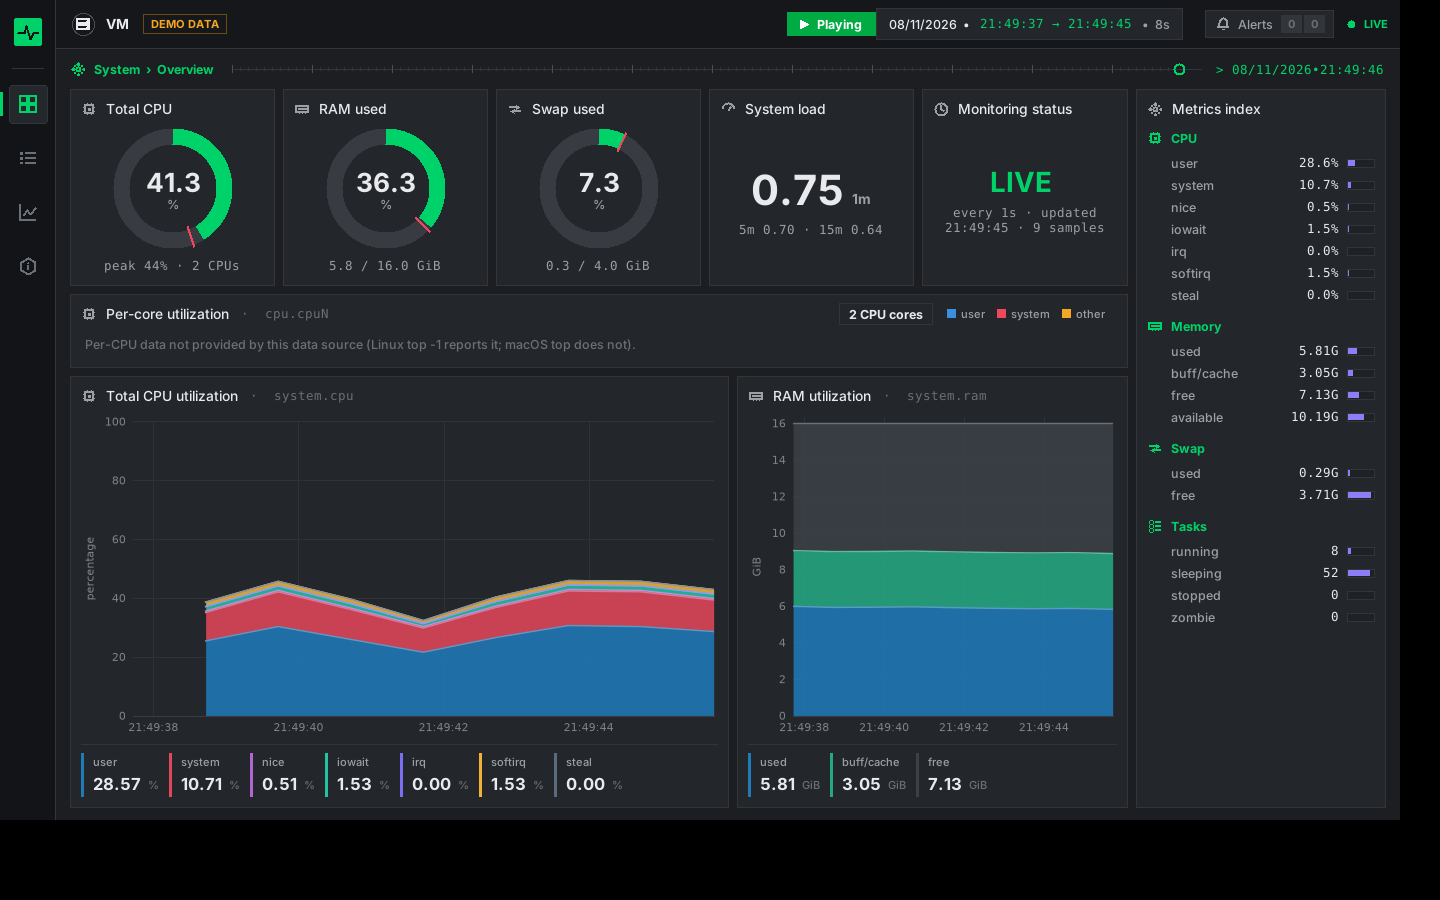
\includegraphics[width=0.95\textwidth]{overview.png}}

{\tiny Overview screen (taken in demo data mode)}
\end{column}
\end{columns}

\vspace{0.5cm}
{\scriptsize \textbf{Team Mentally Unstable}, IIT Dharwad\\
Ankush Tarafdar, Atharv Saxena, Manish Pravin Patil, Chettupelly Dhiren, Pavan}
\end{frame}

% ---------------- Slide 2 ----------------
\begin{frame}{System Architecture}
\begin{columns}[T]
\begin{column}{0.27\textwidth}
\centering
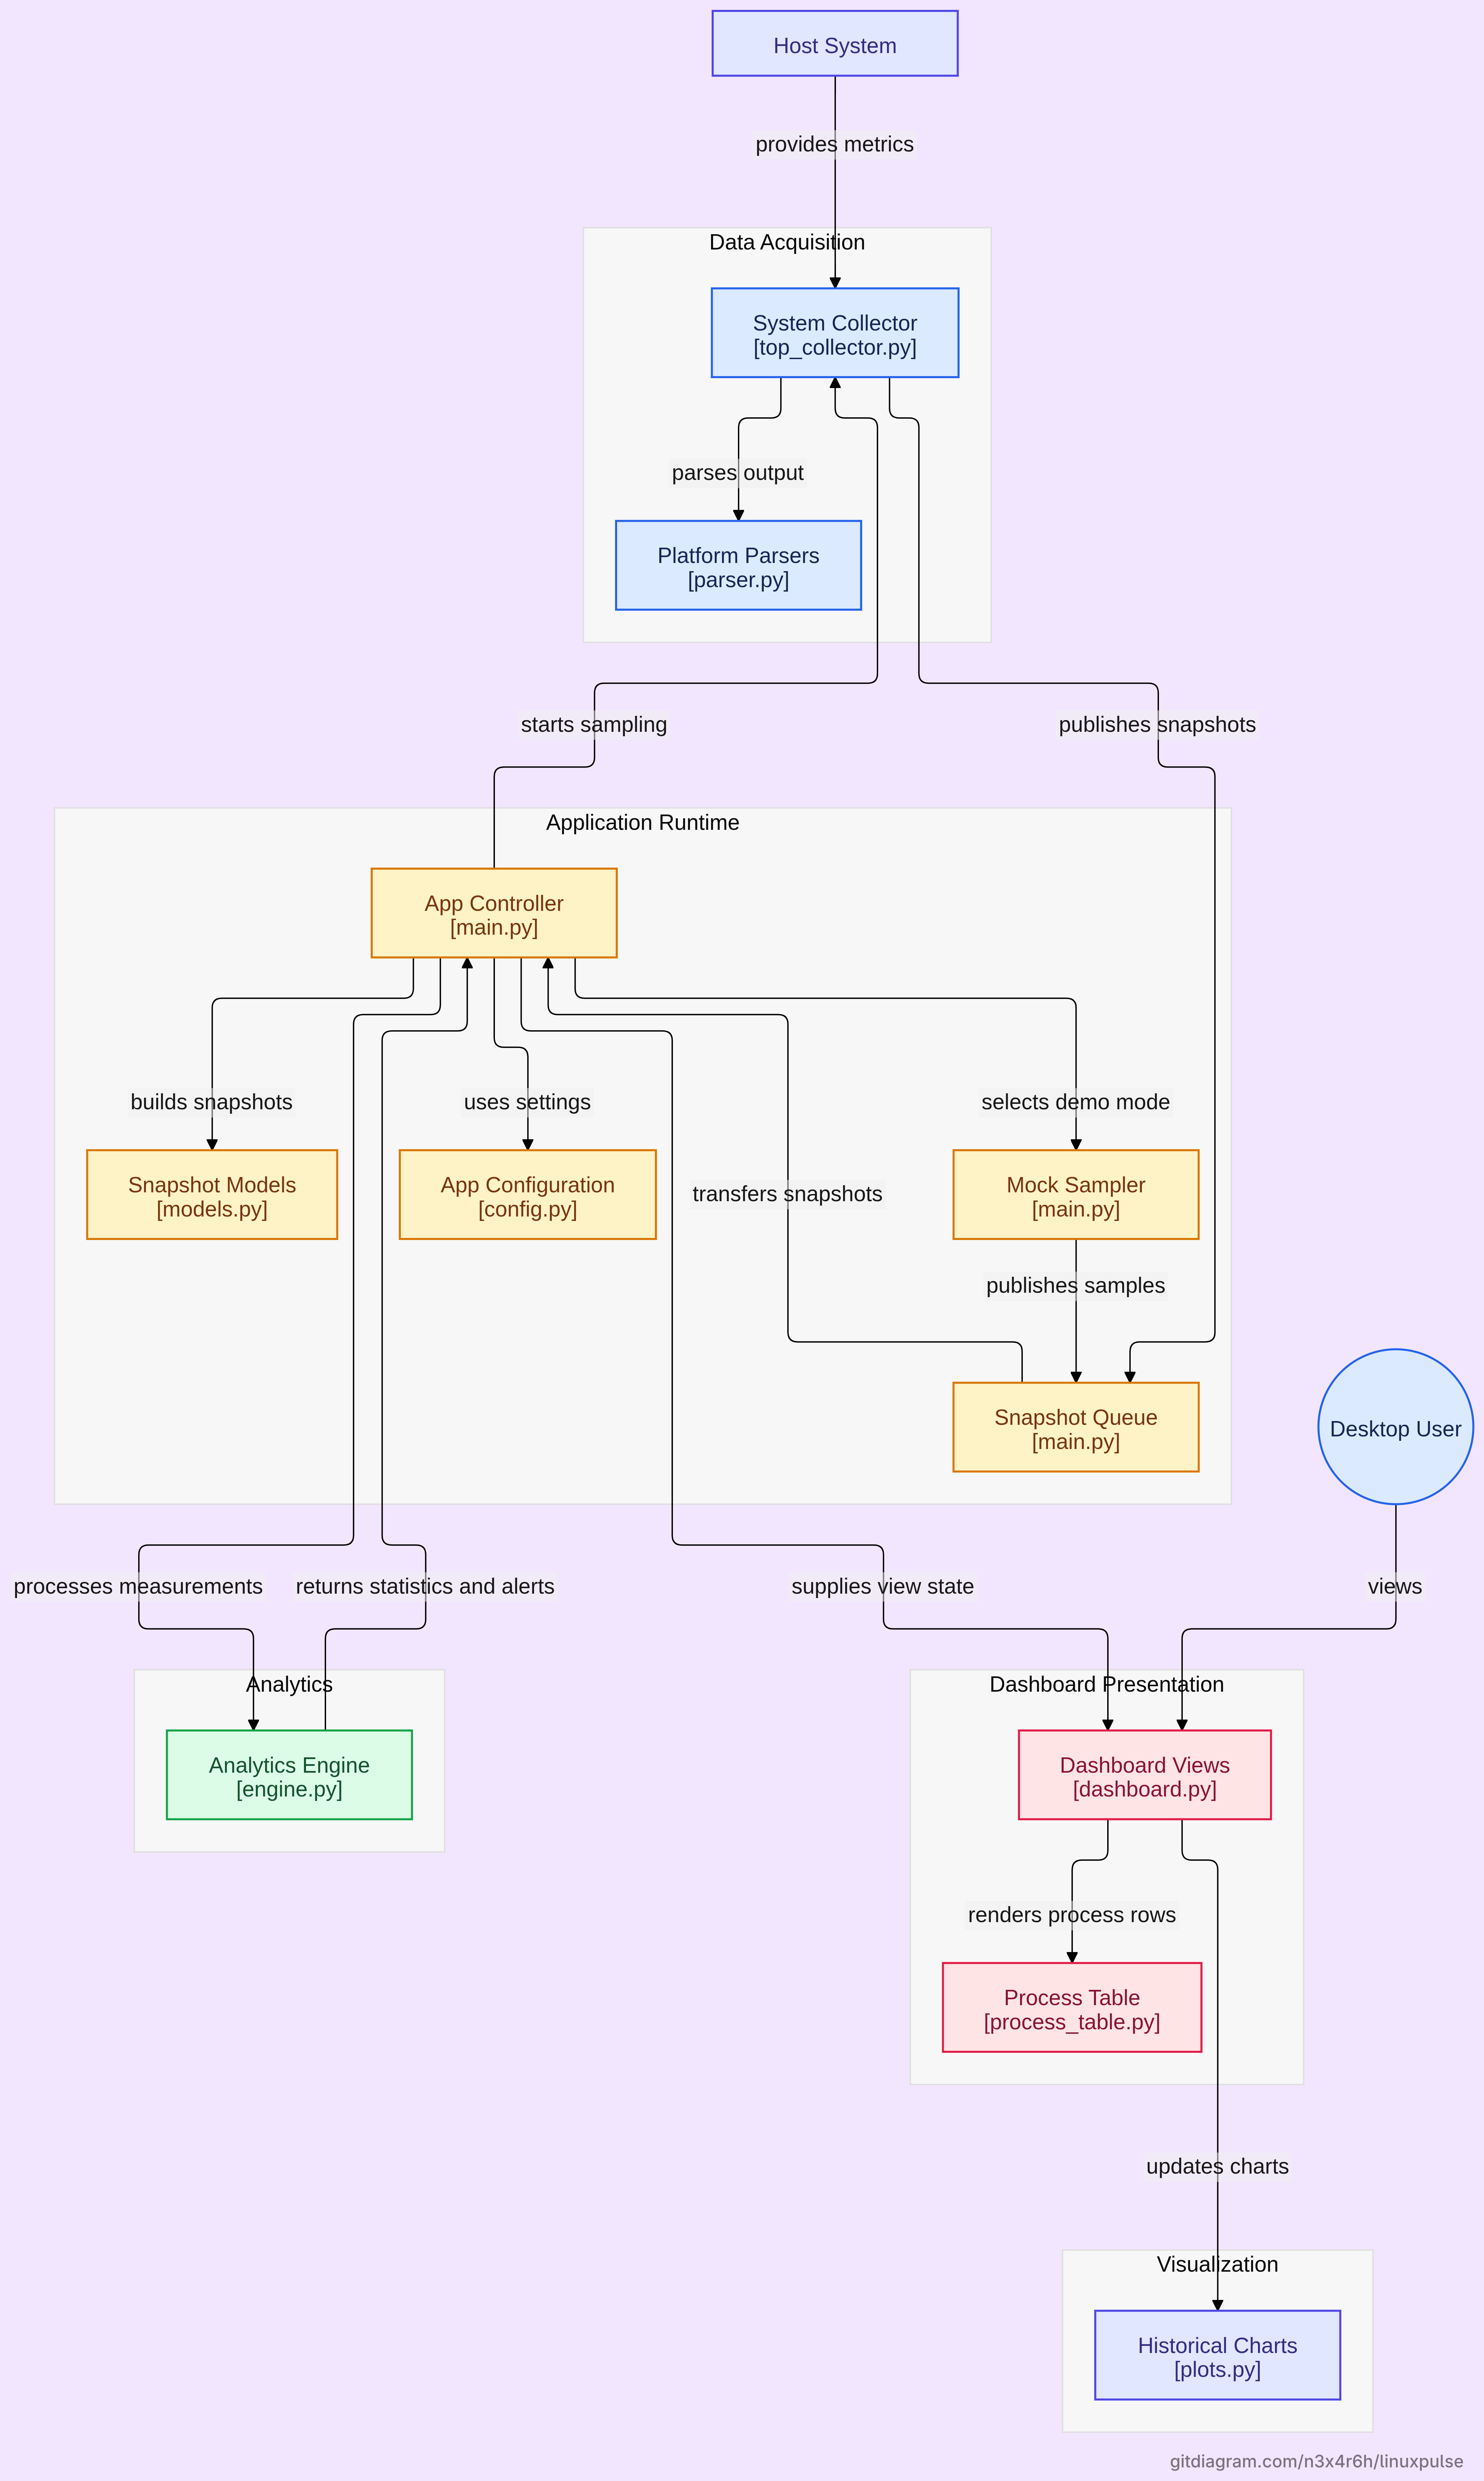
\includegraphics[height=6.6cm]{architecture.png}
\end{column}

\begin{column}{0.71\textwidth}
\textbf{Data flow:}

\vspace{0.1cm}
\small
Host System $\rightarrow$ Collector (\texttt{top\_collector.py}) $\rightarrow$ Parser (\texttt{parser.py})
$\rightarrow$ Application Runtime (\texttt{main.py}) $\rightarrow$ Analytics (\texttt{engine.py})
and Dashboard (\texttt{dashboard.py}) $\rightarrow$ Visualization (\texttt{plots.py})

\vspace{0.3cm}
\begin{itemize}
  \item \textbf{Data acquisition:} the System Collector reads the host and the
        Platform Parsers turn the raw output into structured data
  \item \textbf{Application runtime:} the App Controller builds Snapshot Models,
        reads App Configuration, chooses live data or the Mock Sampler and sends
        results through the Snapshot Queue
  \item \textbf{Analytics:} the engine processes the measurements and returns
        statistics and alerts
  \item \textbf{Dashboard and visualization:} the views show the Process Table
        and update the Historical Charts
\end{itemize}
\end{column}
\end{columns}
\end{frame}

% ---------------- Slide 3 ----------------
\begin{frame}{Data Acquisition and Application Runtime}
\small
\textbf{Pipeline (runs in the collector thread every 2 seconds):}

\vspace{0.1cm}
\fbox{\parbox{0.97\textwidth}{\centering
\texttt{/proc/stat}, \texttt{/proc/meminfo}, \texttt{/proc/loadavg}, \texttt{top -b -n 1} (or \texttt{ps})\\[0.1cm]
$\downarrow$\\
\texttt{top\_collector.py} $\rightarrow$ \texttt{parser.py} $\rightarrow$ \texttt{to\_snapshot()}
$\rightarrow$ \texttt{AnalyticsEngine} $\rightarrow$ \texttt{queue.Queue} (size 256)
$\rightarrow$ Tkinter GUI}}

\vspace{0.3cm}
\begin{columns}[T]
\begin{column}{0.48\textwidth}
\begin{itemize}
  \item \texttt{top\_collector.py}: CPU \% from two \texttt{/proc/stat} readings,
        process list from \texttt{top} in batch mode (\texttt{ps} if that fails)
  \item \texttt{parser.py}: one parsing function for each source, rejects bad input
  \item \texttt{models.py}: dataclasses like \texttt{SystemSnapshot}, \texttt{CPUInfo},
        \texttt{MemoryInfo}, \texttt{SwapInfo}, \texttt{ProcessInfo}
\end{itemize}
\end{column}
\begin{column}{0.48\textwidth}
\begin{itemize}
  \item \texttt{main.py}: the \texttt{Controller} checks each module's output and
        sends the newest state to the GUI; errors are shown as \texttt{SourceError}
  \item \texttt{config.py}: \texttt{AppConfig} holds interval, history size,
        thresholds and queue size
  \item \textbf{Live / mock:} \texttt{--mock} uses \texttt{DemoCollector}, which gives
        the same data format and is labelled DEMO DATA
\end{itemize}
\end{column}
\end{columns}
\end{frame}

% ---------------- Slide 4 ----------------
\begin{frame}{Analytics and Dashboard}
\begin{columns}[T]
\begin{column}{0.49\textwidth}
\begin{block}{Analytics engine (\texttt{engine.py})}
\footnotesize
\begin{itemize}
  \item History in a \texttt{deque(maxlen=300)} with an \texttt{RLock}
  \item Current, mean, min, peak and 10-sample rolling mean
  \item Top processes using \texttt{heapq.nlargest}
  \item Alert when a value $\geq$ its threshold
\end{itemize}
{\tiny Written in plain Python. NumPy is in \texttt{requirements.txt} but not used.}
\end{block}
\end{column}
\begin{column}{0.49\textwidth}
\begin{block}{Interface (Tkinter + Matplotlib)}
\footnotesize
\begin{itemize}
  \item \texttt{dashboard.py}: Overview, Processes and Analytics screens, alert counter and alert lists
  \item \texttt{process\_table.py}: \texttt{ttk.Treeview} with sort, search and filters
  \item \texttt{plots.py}: Matplotlib charts embedded with \texttt{FigureCanvasTkAgg}
\end{itemize}
\end{block}
\end{column}
\end{columns}

\vspace{0.2cm}
\begin{columns}[T]
\begin{column}{0.25\textwidth}
\fbox{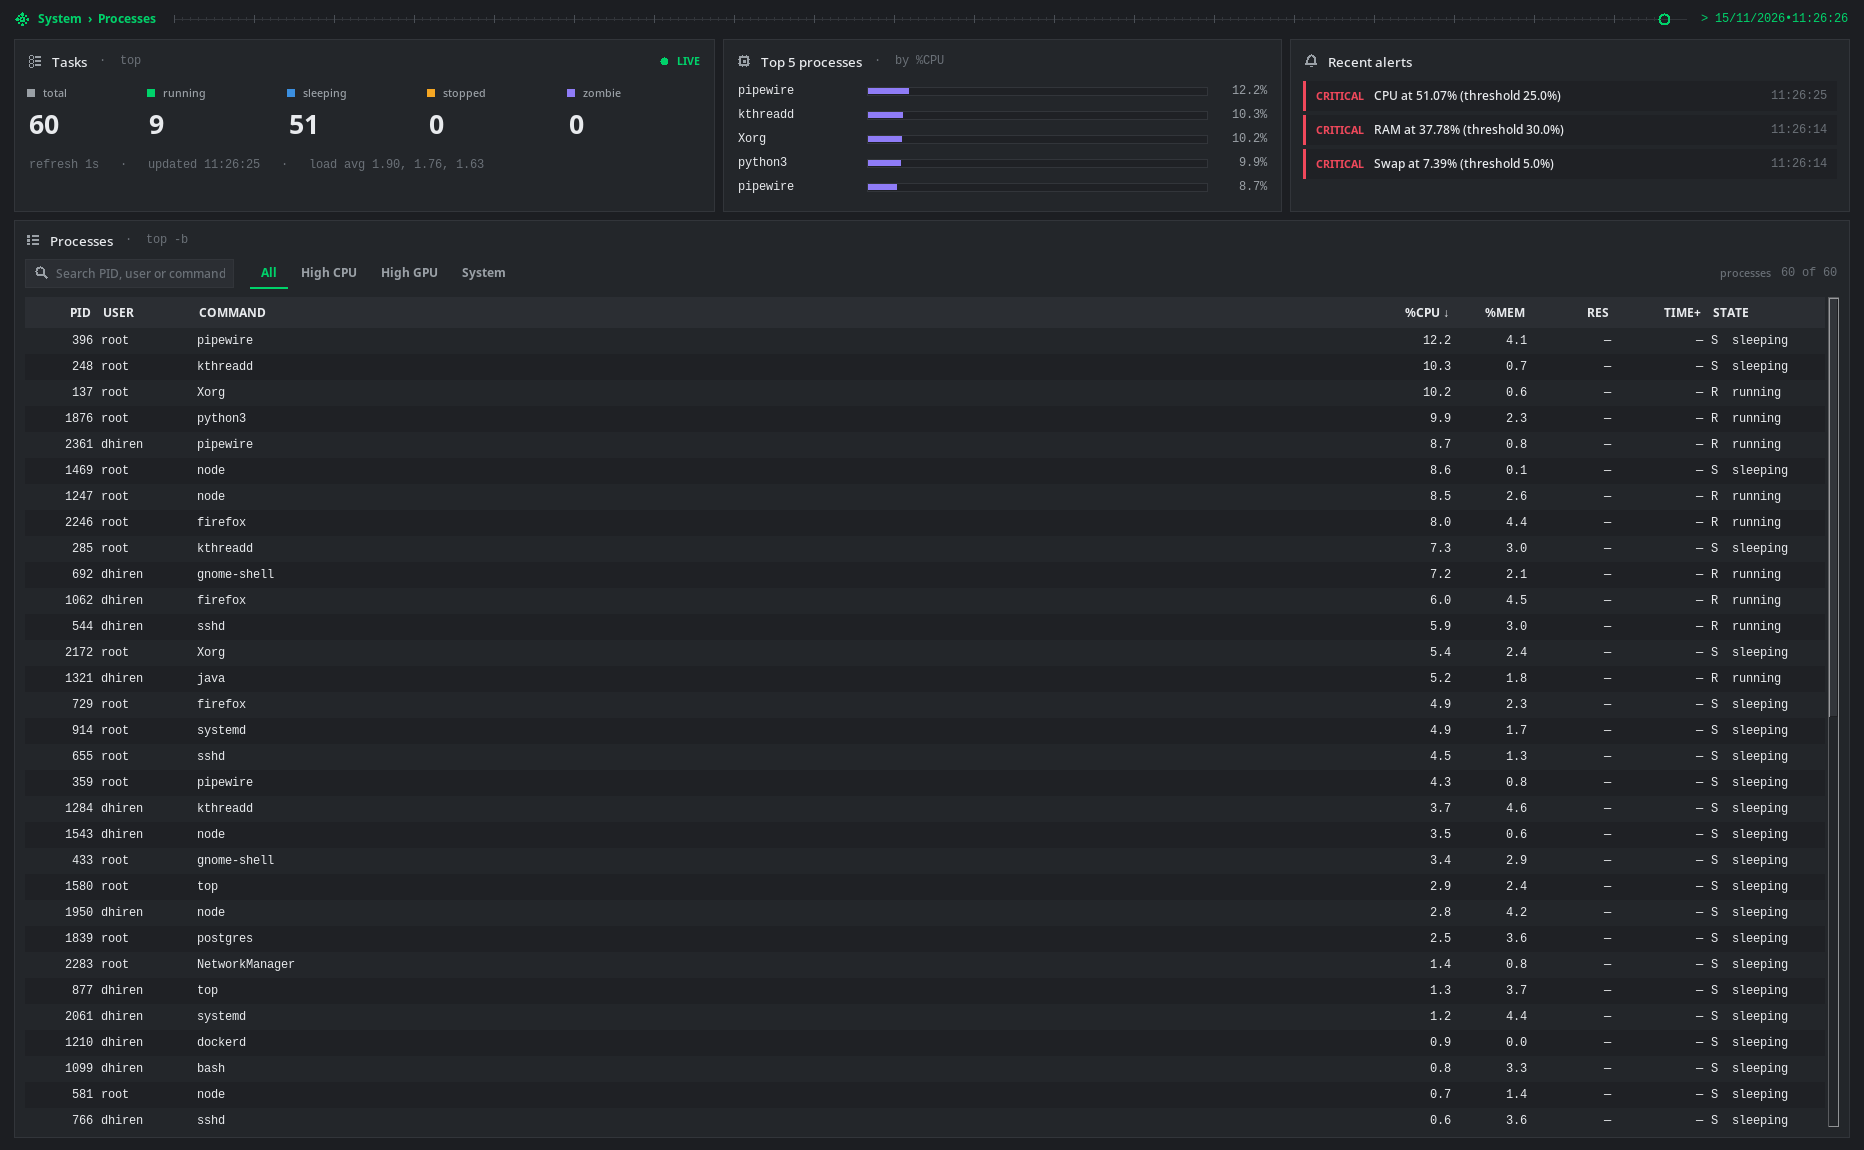
\includegraphics[width=0.93\textwidth]{alerts_processes.png}}

{\tiny Processes screen with alerts}
\end{column}
\begin{column}{0.25\textwidth}
\fbox{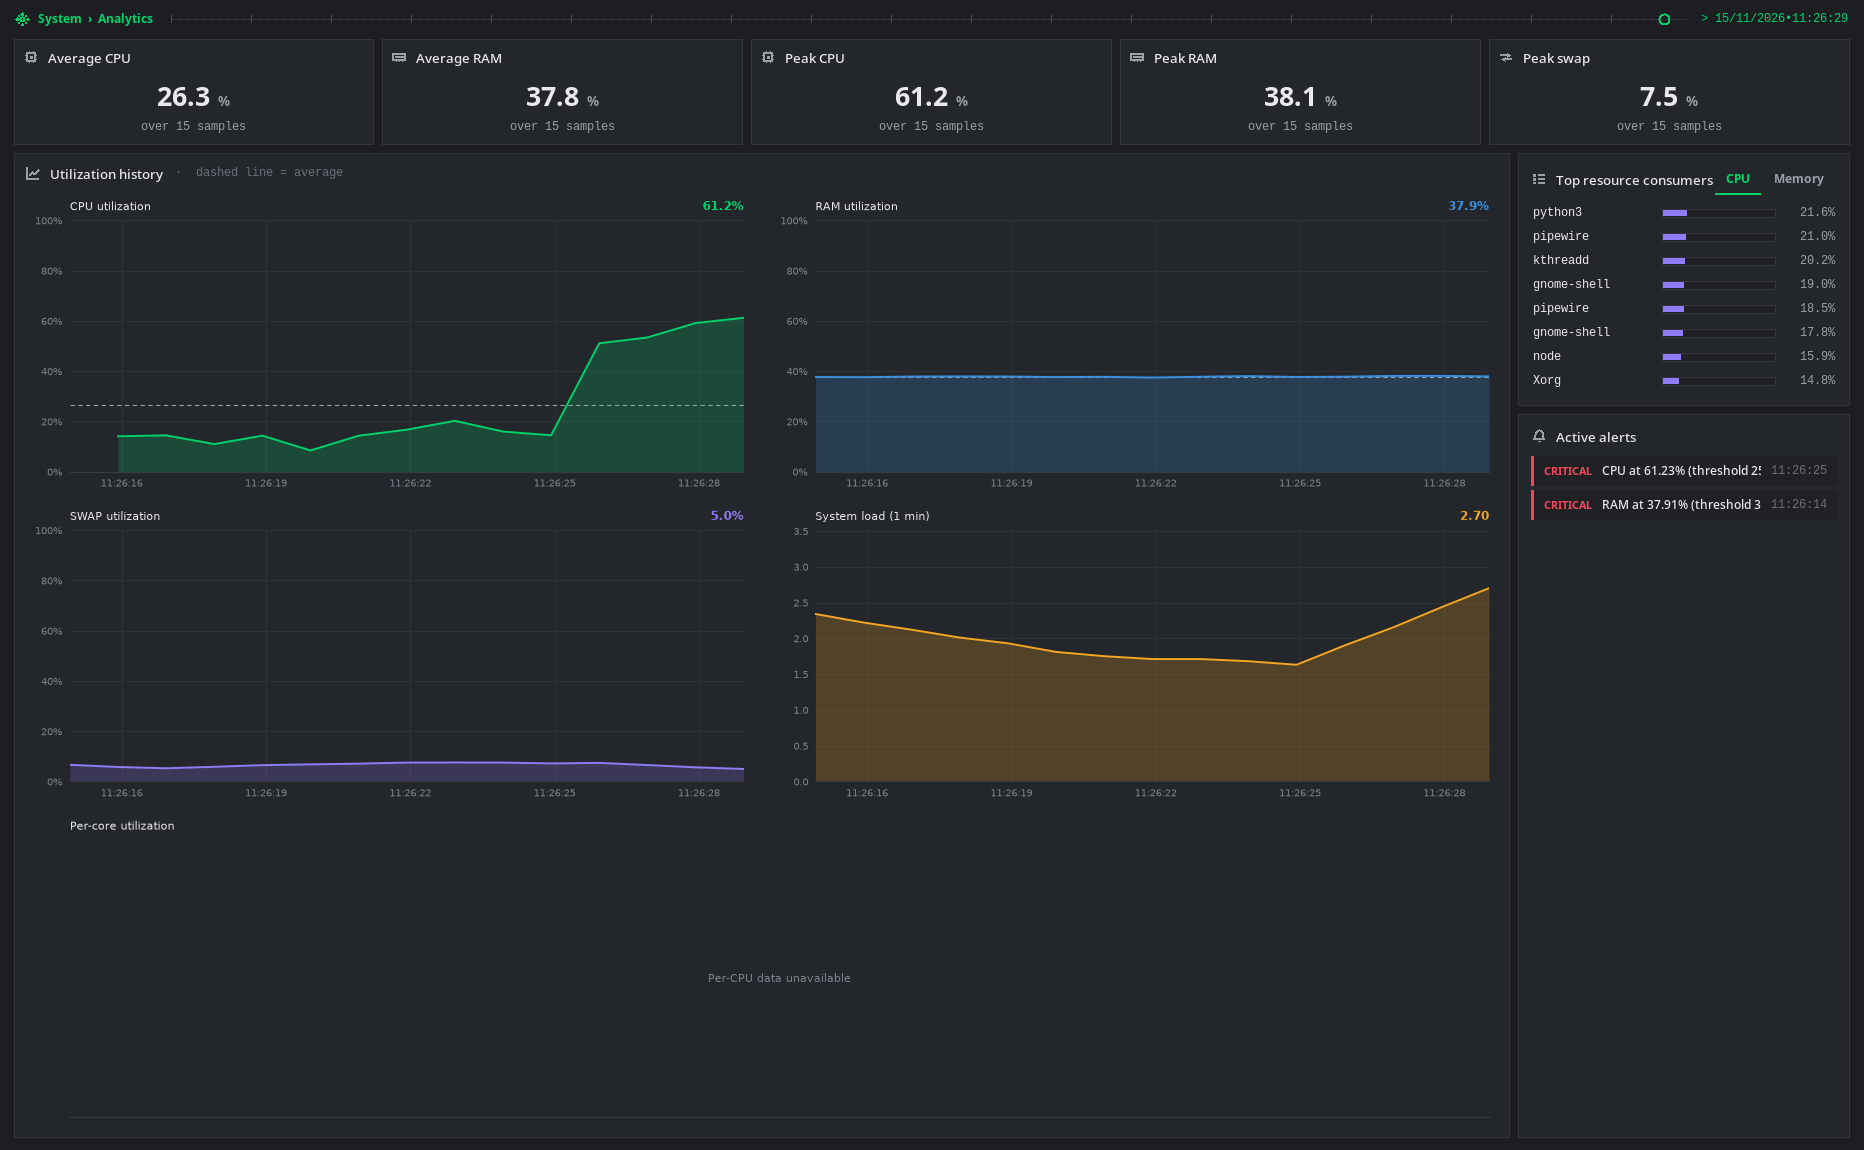
\includegraphics[width=0.93\textwidth]{alerts_analytics.png}}

{\tiny Analytics screen with alerts}
\end{column}
\begin{column}{0.44\textwidth}
\textbf{\scriptsize Threshold warnings} \hfill 
\includegraphics[height=0.35cm]{alerts_badge.png}

\fbox{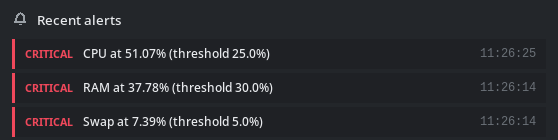
\includegraphics[width=0.96\textwidth]{alerts_panel.png}}

{\tiny For these pictures we lowered the thresholds (CPU 25\%, RAM 30\%, swap 5\%)
so the demo data would trigger alerts. Normal values are 80 / 85 / 80\%.}
\end{column}
\end{columns}
\end{frame}

% ---------------- Slide 5 ----------------
\begin{frame}{Integration, Testing and Performance Profiling}
\begin{columns}[T]

\begin{column}{0.30\textwidth}
\textbf{Concurrency}
\scriptsize

\vspace{0.1cm}
\fbox{\parbox{0.9\textwidth}{\centering \textbf{Collector thread}\\ collect, analyse, make \texttt{ViewState}}}\\
\centering $\downarrow$\\
\fbox{\parbox{0.9\textwidth}{\centering \textbf{\texttt{queue.Queue(256)}}\\ drops the oldest item if full}}\\
$\downarrow$\\
\fbox{\parbox{0.9\textwidth}{\centering \textbf{Tkinter main thread}\\ \texttt{root.after(250 ms)} takes the newest state and updates the widgets and charts}}

\raggedright
\vspace{0.2cm}
Only the main thread changes the GUI. On exit we use \texttt{threading.Event} and \texttt{join()}.
\end{column}

\begin{column}{0.28\textwidth}
\textbf{Testing}
\scriptsize

\vspace{0.1cm}
\begin{tabular}{lr}
\toprule
\texttt{unittest} file & tests \\
\midrule
\texttt{test\_parser} & 20 \\
\texttt{test\_collector} & 10 \\
\texttt{test\_analytics} & 21 \\
\texttt{test\_visualization} & 4 \\
\texttt{test\_controller} & 32 \\
\texttt{test\_integration} & 29 \\
\texttt{test\_gui\_integration} & 4 \\
\midrule
\textbf{Total (all pass)} & \textbf{120} \\
\bottomrule
\end{tabular}

\vspace{0.2cm}
\textbf{Make targets:} install, check, run, mock, test, profile, clean
\end{column}

\begin{column}{0.38\textwidth}
\textbf{C++ benchmark with gprof}
\scriptsize

\vspace{0.1cm}
\texttt{g++ -O0 -pg} $\rightarrow$ run $\rightarrow$ \texttt{gmon.out} $\rightarrow$ \texttt{gprof}
$\rightarrow$ find hot spot $\rightarrow$ optimise and profile again

\vspace{0.2cm}
\texttt{top\_processes} took \textbf{43.7\%} of the time because it copied and fully sorted
every process. We changed it to \texttt{std::partial\_sort} on indices.

\vspace{0.2cm}
\begin{tabular}{lrrr}
\toprule
median of 5 runs & before & after & speed-up \\
\midrule
ranking & 0.843 s & 0.042 s & 20.1x \\
whole program & 1.424 s & 0.603 s & 2.36x \\
\bottomrule
\end{tabular}

\vspace{0.2cm}
\fbox{\parbox{0.95\textwidth}{\textbf{Note:} this is a separate C++ test program.
gprof does not profile the Python dashboard. Both versions give the same output.}}
\end{column}

\end{columns}
\end{frame}

% ---------------- Slide 6 ----------------
\begin{frame}{Team Contributions and Conclusion}
\scriptsize
\setlength{\tabcolsep}{4pt}
\begin{tabular}{|>{\raggedright}p{2.45cm}|>{\raggedright}p{2.45cm}|>{\raggedright}p{2.45cm}|>{\raggedright}p{2.45cm}|>{\raggedright\arraybackslash}p{2.45cm}|}
\hline
\textbf{Member 1} & \textbf{Member 2} & \textbf{Member 3} & \textbf{Member 4} & \textbf{Member 5} \\
Atharv Saxena & Manish Pravin Patil & Chettupelly Dhiren & Pavan & Ankush Tarafdar \\
\hline
\textit{System Data Acquisition Engineer} &
\textit{Analytics and Performance Metrics Engineer} &
\textit{GUI and Application Interface Engineer} &
\textit{Visualization and Quality Assurance Engineer} &
\textit{Systems Architect, Integration and Profiling Engineer} \\
\hline
Collector, metric extraction, platform parsing, collector integration &
Analytics engine, statistics, process ranking, threshold alerts &
Tkinter dashboard, interface components, process table &
Historical charts, visualization integration, regression testing, report &
Orchestration, models, configuration, integration, build, C++ profiling \\
\hline
\texttt{top\_collector.py} \texttt{parser.py} &
\texttt{engine.py} &
\texttt{dashboard.py} \texttt{process\_table.py} &
\texttt{plots.py} \texttt{tests/} &
\texttt{main.py} \texttt{models.py} \texttt{config.py} \texttt{Makefile} \\
\hline
\end{tabular}

\vspace{0.1cm}
\centering
Collect (M1) $\rightarrow$ orchestrate (M5) $\rightarrow$ analyse (M2) $\rightarrow$ present (M3) $\rightarrow$ visualise and test (M4)

\raggedright
\vspace{0.2cm}
\begin{columns}[T]
\begin{column}{0.55\textwidth}
\textbf{\small What we achieved}
\begin{itemize}
  \item Modular, read-only monitor with live or labelled mock data
  \item GUI stays responsive (background thread + queue)
  \item 120 tests passing, GNU Make for building and testing
  \item Ranking 20.1x faster in the gprof case study
\end{itemize}
\end{column}
\begin{column}{0.42\textwidth}
\textbf{\small Future work}
\begin{itemize}
  \item Export history to CSV
  \item Disk I/O and network monitoring
  \item Per-core CPU usage
\end{itemize}
\end{column}
\end{columns}
\end{frame}

\end{document}
